\documentclass[10pt,a4paper]{article}
\usepackage[T1]{fontenc}
\usepackage{lmodern}
\usepackage{microtype}
\usepackage{graphicx}
\usepackage{booktabs}
\usepackage{geometry}
\usepackage{caption}
\usepackage{tikz}
\usepackage{amsfonts}
\usetikzlibrary{arrows.meta}
\definecolor{diagramSource}{HTML}{70828D}
\definecolor{diagramSourceBg}{HTML}{F2F6F7}
\definecolor{diagramEncoder}{HTML}{327886}
\definecolor{diagramEncoderBg}{HTML}{E8F2F3}
\definecolor{diagramHead}{HTML}{AF704D}
\definecolor{diagramHeadBg}{HTML}{FAF0E9}
\definecolor{diagramOp}{HTML}{687688}
\definecolor{diagramOpBg}{HTML}{F0F1F5}
\definecolor{diagramFlow}{HTML}{46545B}
\definecolor{diagramNote}{HTML}{57636A}
\geometry{margin=20mm}
\captionsetup{font=small,labelfont=bf}
\setlength{\parskip}{4pt}
\setlength{\parindent}{0pt}
\renewcommand{\topfraction}{0.88}
\renewcommand{\bottomfraction}{0.82}
\renewcommand{\textfraction}{0.06}
\renewcommand{\floatpagefraction}{0.82}

\title{HealthMirror Study Report}
\author{}
\date{}

\begin{document}
\maketitle
\vspace{-2em}

Five studies covered inpatient laboratory trajectories, single-time-point physiological prediction, paired-face laboratory change, postoperative status, and an independent ECG quality-control task. The facial-video studies used patient-recorded videos linked to hospital records. Laboratory aliases and units were harmonized by explicit rules; physiologically distinct fields, including temperature-corrected and uncorrected oxygen pressures, remained separate. Hospital report times were interpreted in Asia/Shanghai and converted to UTC. Absolute video time came from the metadata Session Timestamp; frame timestamps supplied duration and source-clock diagnostics rather than an alternative clinical clock. A face video was matched to the nearest analyte measurement in the same admission within 24 hours of its capture interval. Measurements within the interval had zero temporal distance; otherwise distance was measured from the nearer boundary. Each video contributed at most one label per analyte. Of 2,846 candidate videos, 1,957 videos from 707 patients entered the 24-hour pool before analyte-specific and frame-eligibility filters.

\section{Study 1: Inpatient laboratory trajectories}

\subsection{Cohort and analysis}

This study characterized laboratory measurements independently of facial-video prediction. Valid numerical measurements were grouped by admission. Verified item aliases and simultaneous duplicate results were collapsed before analysis. Its main settings were:
\begin{itemize}
\setlength{\itemsep}{1pt}
\item \textbf{Analysis unit:} one admission for trajectory summaries, with one median first-to-last change per patient for inference.
\item \textbf{Inference:} two-sided Wilcoxon signed-rank tests, Benjamini--Hochberg false-discovery-rate correction, and 2,000 patient-level bootstrap replicates for median-change intervals.
\item \textbf{Surgical alignment:} measurements aligned to verified coronary artery bypass grafting (CABG) times; other valid principal surgeries were considered separately.
\end{itemize}

\subsection{Observed trajectories}

The analysis retained 838 patients, 1,007 admissions, and 520,726 numerical measurements after harmonization. Of 79 variables with sufficient paired observations, 62 had a patient-level first-to-last comparison with adjusted $q<0.05$. Valid CABG times were available for 769 episodes. Selected CABG-aligned analytes are shown in Fig.~\ref{fig:cabgtrajectory}. For example, median hemoglobin was 139.25 g/L at 3--7 days before surgery, 119 g/L at 0--6 hours afterward, and 103.25 g/L at 3--7 days afterward. These are phase-specific patient summaries, not necessarily trajectories of the same individuals.

\begin{center}
\begin{minipage}{\linewidth}
\centering
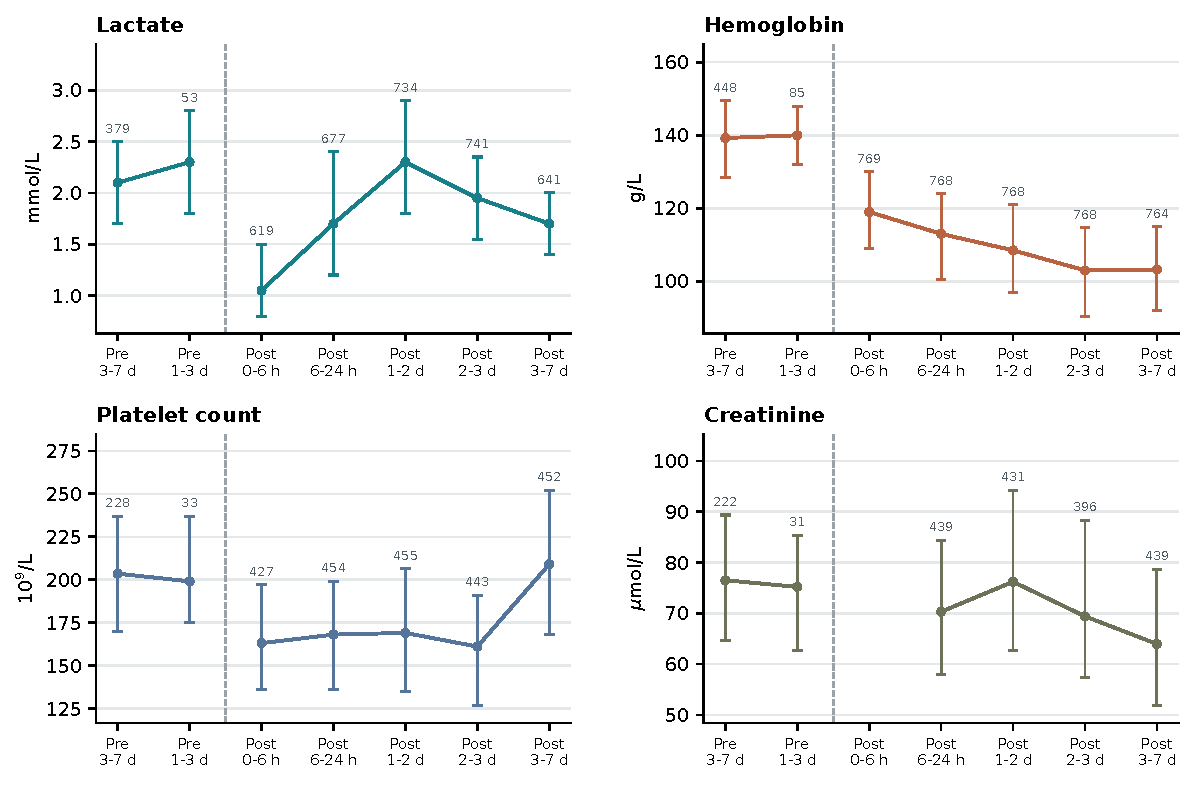
\includegraphics[width=0.96\linewidth]{figures/cabg_selected_trajectories.pdf}
\captionof{figure}{Selected CABG-aligned laboratory values. Points are patient-balanced phase medians, whiskers are interquartile ranges, and numbers above them are patients contributing to each phase. The dashed line separates pre- and postoperative phases; line segments are not connected across surgery. Phase cohorts can differ. Cells with fewer than 20 patients are omitted, including creatinine at postoperative 0--6 hours.}
\label{fig:cabgtrajectory}
\end{minipage}
\end{center}

\section{Study 2: Single-time-point physiological prediction}

\subsection{Tasks, inputs, and training}

Eight analytes were predicted independently: oxyhemoglobin fraction, lactate, urea, total bilirubin, platelet count, hemoglobin, arterial/alveolar oxygen-pressure ratio, and creatinine. Still-face, laboratory-history, fused, and continuous-video models were evaluated on aligned per-analyte task records. Regression targets were original laboratory values scaled with the training partition's median and interquartile range (IQR); predictions were returned to original units. Separate binary models used protocol-defined abnormality thresholds. The model and optimization settings were:
\begin{itemize}
\setlength{\itemsep}{1pt}
\item \textbf{Face-only EfficientNet-B0:} 20 nonadjacent RGB frames per video, resized to $224\times224$, and an ImageNet-pretrained encoder with a 32-unit task head. Each training frame was expanded into original, horizontal-flip, center-crop, brightness-adjusted, and contrast-adjusted views. Validation and test used original frames only; their predictions were averaged per video.
\item \textbf{Laboratory-history controls:} all earlier values of the same analyte in the same admission, each accompanied by elapsed time to the target event. A lightweight per-event encoder was mean-pooled; its output was used alone or concatenated with face features before a 32-unit head. The target event itself was excluded from history.
\item \textbf{Continuous-video R3D-18:} up to three nonoverlapping, source-contiguous 16-frame clips per video, center-cropped from $128\times128$ to $112\times112$ without temporal resampling. A Kinetics-pretrained R3D-18 with a 32-unit head saw one sampled clip per training epoch; all indexed clips were averaged for video-level evaluation.
\item \textbf{Optimization:} face regression used Smooth L1 loss. Its frozen-backbone head stage used a learning rate of $2\times10^{-4}$ for up to 40 epochs, followed by full-encoder fine-tuning at $10^{-5}$ for up to 60 epochs, both with validation-based early stopping. Binary classification used weighted binary cross-entropy, training-only positive-class weights, and a fixed 0.5 decision threshold. The video model used the same two-stage pattern with learning rates $10^{-3}$ and $10^{-5}$. A face-only patient-diverse-batch variant used 30/40-epoch limits and learning rates $10^{-4}/3\times10^{-6}$.
\end{itemize}

\begin{center}
\begin{minipage}{\linewidth}
\centering
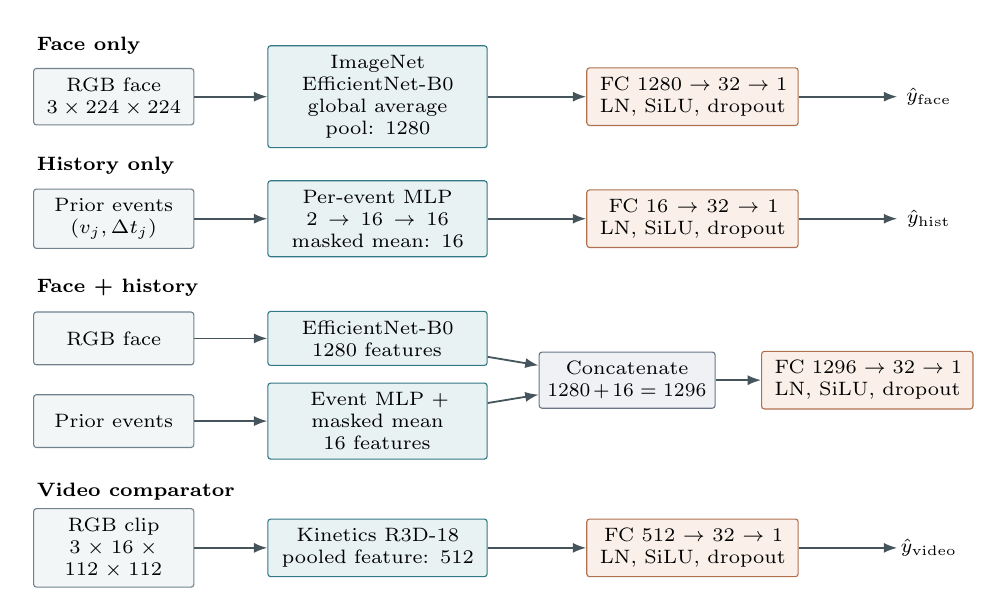
\begin{tikzpicture}[
    x=1cm,y=1cm,>=Latex,
    every node/.style={font=\scriptsize,align=center},
    source/.style={draw=diagramSource,fill=diagramSourceBg,rounded corners=1pt,minimum height=0.67cm,text width=1.8cm},
    encoder/.style={draw=diagramEncoder,fill=diagramEncoderBg,rounded corners=1pt,minimum height=0.67cm,text width=2.55cm},
    head/.style={draw=diagramHead,fill=diagramHeadBg,rounded corners=1pt,minimum height=0.67cm,text width=2.45cm},
    op/.style={draw=diagramOp,fill=diagramOpBg,rounded corners=1pt,minimum height=0.67cm,text width=2.0cm},
    flow/.style={-{Latex[length=1.7mm]},draw=diagramFlow,line width=0.65pt}
]
\node[anchor=west,font=\bfseries\scriptsize] at (0,4.65) {Face only};
\node[source] (face) at (1.1,4.0) {RGB face\\$3\times224\times224$};
\node[encoder] (faceenc) at (4.45,4.0) {ImageNet EfficientNet-B0\\global average pool: 1280};
\node[head] (facehead) at (8.45,4.0) {FC $1280\to32\to1$\\LN, SiLU, dropout};
\node at (11.45,4.0) {$\hat y_{\rm face}$};
\draw[flow] (face) -- (faceenc);
\draw[flow] (faceenc) -- (facehead);
\draw[flow] (facehead) -- (11.05,4.0);

\node[anchor=west,font=\bfseries\scriptsize] at (0,3.12) {History only};
\node[source] (hist) at (1.1,2.45) {Prior events\\$(v_j,\Delta t_j)$};
\node[encoder] (histenc) at (4.45,2.45) {Per-event MLP $2\to16\to16$\\masked mean: 16};
\node[head] (histhead) at (8.45,2.45) {FC $16\to32\to1$\\LN, SiLU, dropout};
\node at (11.45,2.45) {$\hat y_{\rm hist}$};
\draw[flow] (hist) -- (histenc);
\draw[flow] (histenc) -- (histhead);
\draw[flow] (histhead) -- (11.05,2.45);

\node[anchor=west,font=\bfseries\scriptsize] at (0,1.57) {Face + history};
\node[source] (fuseface) at (1.1,0.93) {RGB face};
\node[source] (fusehist) at (1.1,-0.12) {Prior events};
\node[encoder] (fuseenc) at (4.45,0.93) {EfficientNet-B0\\1280 features};
\node[encoder] (fusemlp) at (4.45,-0.12) {Event MLP + masked mean\\16 features};
\node[op] (concat) at (7.62,0.40) {Concatenate\\$1280+16=1296$};
\node[head] (fusehead) at (10.67,0.40) {FC $1296\to32\to1$\\LN, SiLU, dropout};
\draw[flow] (fuseface) -- (fuseenc);
\draw[flow] (fusehist) -- (fusemlp);
\draw[flow] (fuseenc) -- (concat);
\draw[flow] (fusemlp) -- (concat);
\draw[flow] (concat) -- (fusehead);

\node[anchor=west,font=\bfseries\scriptsize] at (0,-1.02) {Video comparator};
\node[source] (clip) at (1.1,-1.73) {RGB clip\\$3\times16\times112\times112$};
\node[encoder] (r3d) at (4.45,-1.73) {Kinetics R3D-18\\pooled feature: 512};
\node[head] (videohead) at (8.45,-1.73) {FC $512\to32\to1$\\LN, SiLU, dropout};
\node at (11.45,-1.73) {$\hat y_{\rm video}$};
\draw[flow] (clip) -- (r3d);
\draw[flow] (r3d) -- (videohead);
\draw[flow] (videohead) -- (11.05,-1.73);
\end{tikzpicture}

\captionof{figure}{Study 2 model families. Each analyte has a separate scalar model and head; the four rows are independent protocols, not branches of one jointly trained network. The face and history variants use original-value regression or separate binary heads with the same feature dimensions. LN denotes layer normalization.}
\label{fig:singlearch}
\end{minipage}
\end{center}

Original experiments used distribution-selected, patient-disjoint training/validation/test splits near 60/20/20. Standard face regression, patient-diverse face regression, video regression, and face classification also shared a five-fold evaluation. For each analyte, one patient fold was test, the next validation, and the other three training; a 256-candidate search balanced value distributions, abnormality rates, and fold sizes. Training-only scalers and positive-class weights were refitted in each fold. Each eligible video therefore had one out-of-fold (OOF) prediction per protocol. Regression was assessed by pooled video-level $R^2$, Pearson $r$, and mean absolute error (MAE); binary prediction by area under the receiver operating characteristic curve (AUROC) and balanced accuracy (bACC). The fold search did not enforce the original three-way split's pairwise hard limits, so the five-fold and original-holdout estimates are reported separately.

\subsection{Five-fold findings}

The common five-fold evaluation included 707--1,897 videos per analyte after matching and frame eligibility (Table~\ref{tab:cv}). Hemoglobin had 1,897 videos; urea and creatinine each had 707. These are video counts rather than independent-patient counts.

Face-only EfficientNet-B0 regression reached pooled OOF $R^2=0.244$ for hemoglobin and $0.116$ for lactate. The patient-diverse variant yielded $0.260$ and $0.148$; R3D-18 video yielded $0.197$ and $0.063$ on the same task records and folds. Platelet count and urea had near-zero or negative $R^2$ under all three protocols (Fig.~\ref{fig:cvreg}). There was no uniform gain from continuous video over selected still frames.

Face-only binary prediction achieved pooled OOF AUROC/bACC of $0.778/0.714$ for hemoglobin, $0.632/0.596$ for lactate, and $0.627/0.592$ for bilirubin. Platelet count, oxyhemoglobin fraction, and A/a PO$_2$ ratio had bACC near $0.5$ at the fixed threshold (Fig.~\ref{fig:cvclass}).

\begin{table}[bp]
\centering
\caption{Pooled five-fold OOF performance for matched single-time-point tasks. Regression columns are video-level $R^2$; binary columns describe a separately trained face-only classifier. $n$ counts videos.}
\label{tab:cv}
\small
\setlength{\tabcolsep}{3.5pt}
\begin{tabular}{lrrrrrr}
\toprule
& & \multicolumn{3}{c}{Regression $R^2$} & \multicolumn{2}{c}{Face-only classification} \\
\cmidrule(lr){3-5}\cmidrule(lr){6-7}
Target & $n$ & \shortstack{Face-only\\EfficientNet-B0} & \shortstack{Patient-diverse\\EfficientNet-B0} & \shortstack{Video\\R3D-18} & AUROC & bACC \\
\midrule
Hemoglobin & 1,897 & 0.244 & 0.260 & 0.197 & 0.778 & 0.714 \\
Lactate & 1,336 & 0.116 & 0.148 & 0.063 & 0.632 & 0.596 \\
Oxyhemoglobin & 1,346 & 0.088 & 0.088 & 0.073 & 0.508 & 0.504 \\
A/a PO2 ratio & 1,410 & 0.064 & 0.109 & 0.049 & 0.532 & 0.497 \\
Bilirubin & 733 & -0.009 & 0.009 & -0.007 & 0.627 & 0.592 \\
Creatinine & 707 & -0.011 & 0.004 & 0.002 & 0.542 & 0.517 \\
Urea & 707 & -0.029 & -0.047 & -0.020 & 0.559 & 0.547 \\
Platelets & 838 & -0.019 & -0.012 & -0.044 & 0.497 & 0.500 \\
\bottomrule

\end{tabular}
\end{table}

\begin{figure}[tbp]
\centering
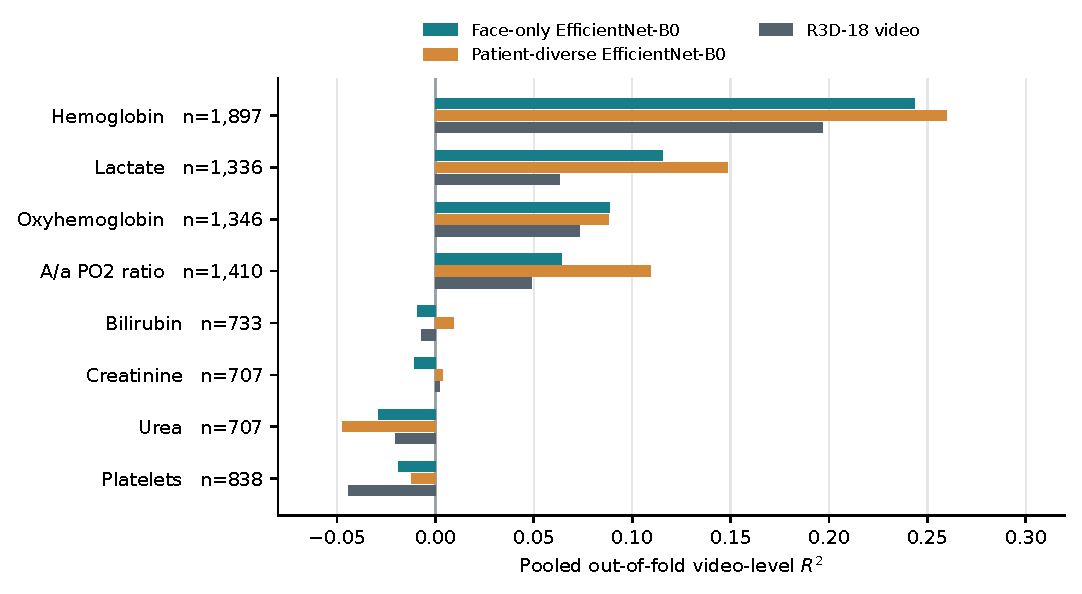
\includegraphics[width=\linewidth]{figures/exp2_exp3_cv_regression.pdf}
\caption{Pooled OOF video-level $R^2$ on identical five-fold task records. Bars distinguish standard face-only EfficientNet-B0, its patient-diverse training variant, and continuous-video R3D-18.}
\label{fig:cvreg}
\end{figure}

\begin{figure}[tbp]
\centering
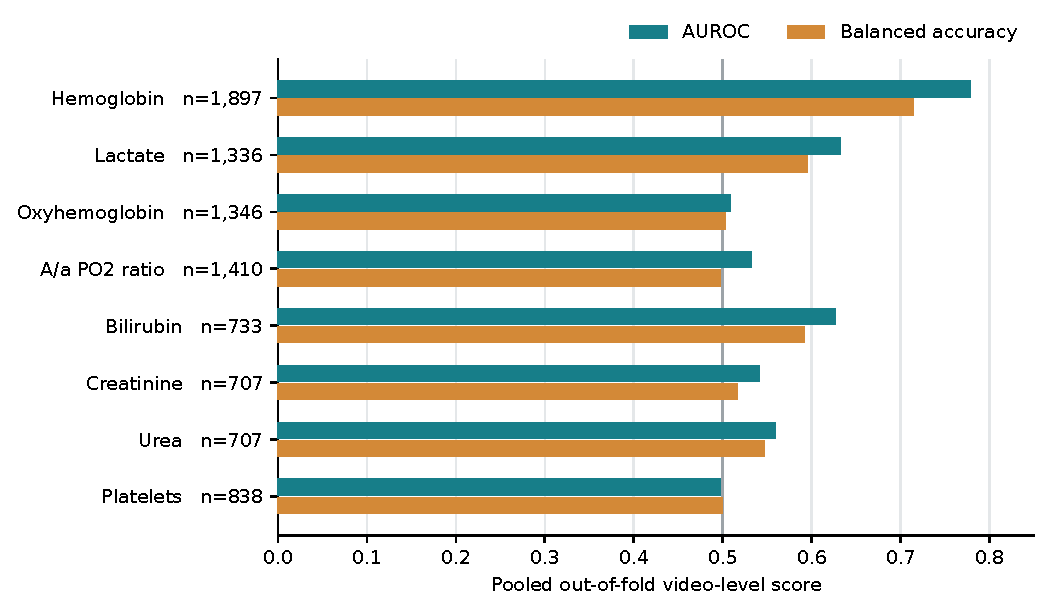
\includegraphics[width=\linewidth]{figures/exp2_cv_classification.pdf}
\caption{Pooled OOF face-only binary prediction. AUROC and bACC are on a 0--1 scale; the vertical line at 0.5 marks chance-level ranking or balanced classification.}
\label{fig:cvclass}
\end{figure}

\subsection{Original-holdout findings and history comparison}

On the original held-out split, face-only hemoglobin AUROC/bACC was $0.720/0.698$ on 366 videos. Figure~\ref{fig:training} shows the original-holdout face-only hemoglobin regressor's epoch-level training and validation losses; the stage boundary separates head training from full-encoder fine-tuning and is not a five-fold average.

For matched original-holdout hemoglobin regression, $R^2$ was $0.164$ for face only, $0.774$ for history only, and $0.770$ for face plus history ($n=366$). MAEs were $14.61$, $7.37$, and $7.49$ g/L, respectively. For creatinine ($n=123$), $R^2$ was $0.021$, $0.150$, and $0.529$ (Fig.~\ref{fig:history}). Corresponding hemoglobin binary AUROC/bACC was $0.720/0.698$ (face), $0.924/0.845$ (history), and $0.905/0.802$ (fusion). In a smaller history-available cohort, median test $R^2$ was $0.076$ for a matched history-only network versus $-0.022$ for sampling-time-only input and $-0.008$ for surgery-time-only input.

\begin{figure}[tbp]
\centering
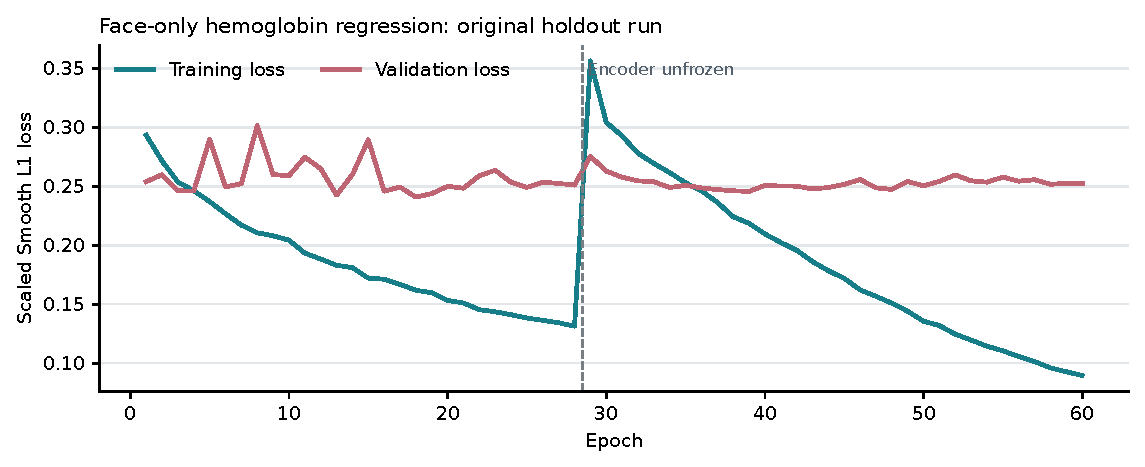
\includegraphics[width=\linewidth]{figures/exp2_hemoglobin_training.pdf}
\caption{Training and validation Smooth L1 loss for the original-holdout face-only hemoglobin regressor. The dashed line marks encoder unfreezing.}
\label{fig:training}
\end{figure}

\begin{figure}[tbp]
\centering
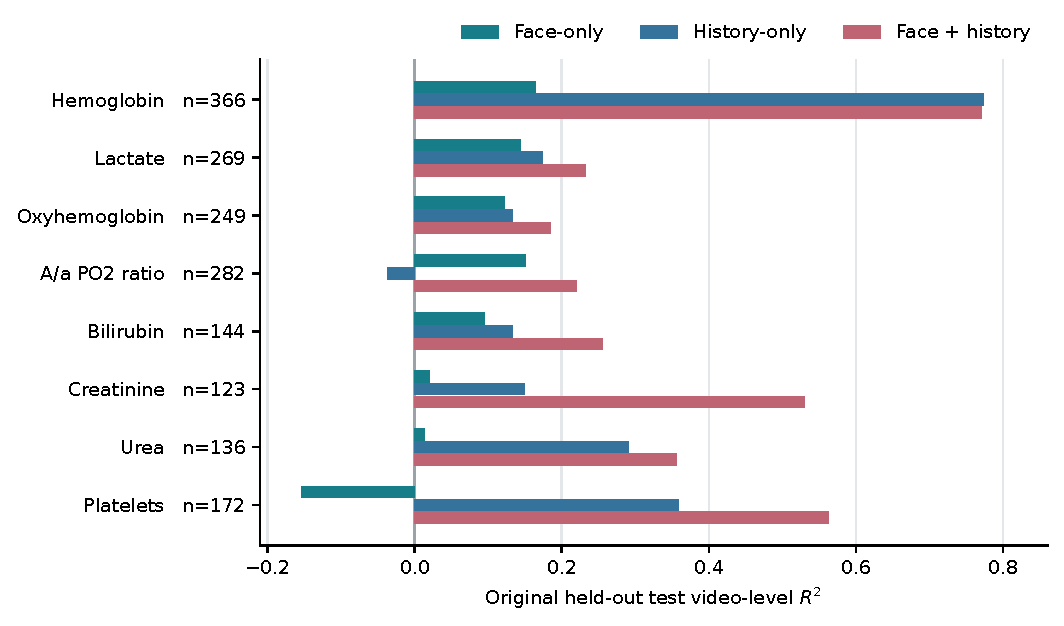
\includegraphics[width=\linewidth]{figures/exp2_history_ablation.pdf}
\caption{Regression $R^2$ for face-only, history-only, and fused models on aligned original held-out test videos. These are not five-fold estimates.}
\label{fig:history}
\end{figure}

\clearpage
\section{Study 3: Paired-face laboratory change}

\subsection{Pair construction and training}

For each analyte, a video was assigned its nearest laboratory event within 24 hours; where several videos selected one event, only the closest video was retained. Consecutive distinct events within a patient formed an ordered pair if both event and video times increased. The nine targets comprised Study 2's eight analytes plus troponin. Key settings were:
\begin{itemize}
\setlength{\itemsep}{1pt}
\item \textbf{Regression target:} later minus earlier canonical laboratory value, robust-scaled with the training-pair median and IQR.
\item \textbf{Inputs and model:} 20 nonadjacent frame pairs per ordered video pair with five synchronized training views. One shared ImageNet-pretrained EfficientNet-B0 encoded both faces; later-minus-earlier feature differences entered a 32-unit scalar head.
\item \textbf{Training and evaluation:} frozen-encoder head training at $2\times10^{-4}$ for at most 40 epochs, then full fine-tuning at $10^{-5}$ for at most 60 epochs. The distribution-selected patient split was near 60/20/20. Original-view frame-pair predictions were averaged to one event-pair prediction.
\item \textbf{Direction task:} a separately trained weighted binary classifier predicted whether the later value was strictly higher. Exact ties were removed; positive-class weights came from training pairs, and test probabilities used a fixed 0.5 cutoff.
\end{itemize}

\begin{center}
\begin{minipage}{\linewidth}
\centering
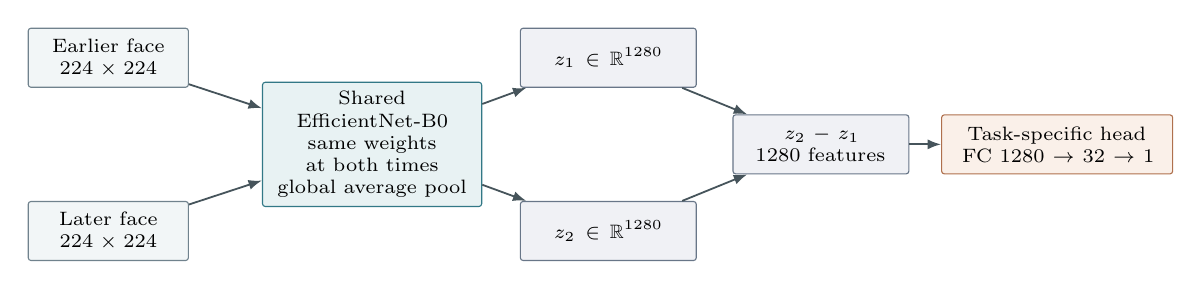
\begin{tikzpicture}[
    x=1cm,y=1cm,>=Latex,
    every node/.style={font=\scriptsize,align=center},
    source/.style={draw=diagramSource,fill=diagramSourceBg,rounded corners=1pt,minimum height=0.75cm,text width=1.8cm},
    encoder/.style={draw=diagramEncoder,fill=diagramEncoderBg,rounded corners=1pt,minimum height=1.05cm,text width=2.55cm},
    op/.style={draw=diagramOp,fill=diagramOpBg,rounded corners=1pt,minimum height=0.75cm,text width=2.0cm},
    head/.style={draw=diagramHead,fill=diagramHeadBg,rounded corners=1pt,minimum height=0.75cm,text width=2.7cm},
    flow/.style={-{Latex[length=1.7mm]},draw=diagramFlow,line width=0.65pt}
]
\node[source] (early) at (1.0,1.1) {Earlier face\\$224\times224$};
\node[source] (late) at (1.0,-1.1) {Later face\\$224\times224$};
\node[encoder] (shared) at (4.35,0) {Shared EfficientNet-B0\\same weights at both times\\global average pool};
\node[op] (zearly) at (7.35,1.1) {$z_1\in\mathbb{R}^{1280}$};
\node[op] (zlate) at (7.35,-1.1) {$z_2\in\mathbb{R}^{1280}$};
\node[op] (diff) at (10.05,0) {$z_2-z_1$\\1280 features};
\node[head] (head) at (13.05,0) {Task-specific head\\FC $1280\to32\to1$};
\draw[flow] (early) -- (shared);
\draw[flow] (late) -- (shared);
\draw[flow] (shared) -- (zearly);
\draw[flow] (shared) -- (zlate);
\draw[flow] (zearly) -- (diff);
\draw[flow] (zlate) -- (diff);
\draw[flow] (diff) -- (head);
\end{tikzpicture}

\captionof{figure}{Study 3 main paired-face model. Both face time points pass through the \emph{same} EfficientNet-B0 weights, and the later-minus-earlier pooled feature enters a task-specific 32-unit head. Regression and up/down classification are trained as separate models with this topology.}
\label{fig:pairarch}
\end{minipage}
\end{center}

A secondary training-free analysis compared frozen face-feature similarity with similarity of held-out laboratory values or changes. It selected one observation per patient and reported Spearman correlation, permutation tests, and false-discovery-rate adjustment. Single-time-point and paired-change cohorts were not paired with one another in this analysis.

\subsection{Change prediction and feature associations}

Paired-face regression was strongest for hemoglobin ($n=182$ held-out event pairs; MAE $10.51$ g/L, $R^2=0.325$, $r=0.571$), lactate ($n=104$; MAE $0.732$ mmol/L, $R^2=0.193$, $r=0.450$), and oxyhemoglobin fraction ($n=105$; $R^2=0.149$). Urea, troponin, platelets, creatinine, and bilirubin had approximately zero or negative test $R^2$ (Table~\ref{tab:change}; Fig.~\ref{fig:change}).

The up/down classifier achieved AUROC/bACC of $0.722/0.607$ for oxyhemoglobin fraction ($n=104$), $0.679/0.610$ for hemoglobin ($n=178$), $0.654/0.612$ for lactate ($n=96$), and $0.663/0.481$ for troponin ($n=122$). Its positive endpoint was a numerical increase, not necessarily a favorable clinical change. Counts differ from regression where exact ties were excluded.

\begin{table}[bp]
\centering
\caption{Original held-out pair-level change prediction. $n_r$ and $n_c$ count regression and binary-classification event pairs; the binary task excludes exact ties.}
\label{tab:change}
\small
\setlength{\tabcolsep}{4pt}
\begin{tabular}{lrrrrrr}
\toprule
& \multicolumn{3}{c}{Change regression} & \multicolumn{3}{c}{Up/down classification} \\
\cmidrule(lr){2-4}\cmidrule(lr){5-7}
Target & $n_r$ & $R^2$ & Pearson $r$ & $n_c$ & AUROC & bACC \\
\midrule
Hemoglobin & 182 & 0.325 & 0.571 & 178 & 0.679 & 0.610 \\
Lactate & 104 & 0.193 & 0.450 & 96 & 0.654 & 0.612 \\
Oxyhemoglobin & 105 & 0.149 & 0.386 & 104 & 0.722 & 0.607 \\
A/a PO2 ratio & 112 & 0.038 & 0.223 & 112 & 0.512 & 0.494 \\
Bilirubin & 56 & -0.002 & 0.079 & 56 & 0.509 & 0.505 \\
Troponin & 122 & -0.007 & -0.018 & 122 & 0.663 & 0.481 \\
Creatinine & 55 & -0.059 & -0.025 & 54 & 0.619 & 0.588 \\
Urea & 58 & -0.158 & -0.072 & 58 & 0.363 & 0.426 \\
Platelets & 73 & -0.077 & 0.032 & 72 & 0.578 & 0.540 \\
\bottomrule

\end{tabular}
\end{table}

\begin{figure}[tbp]
\centering
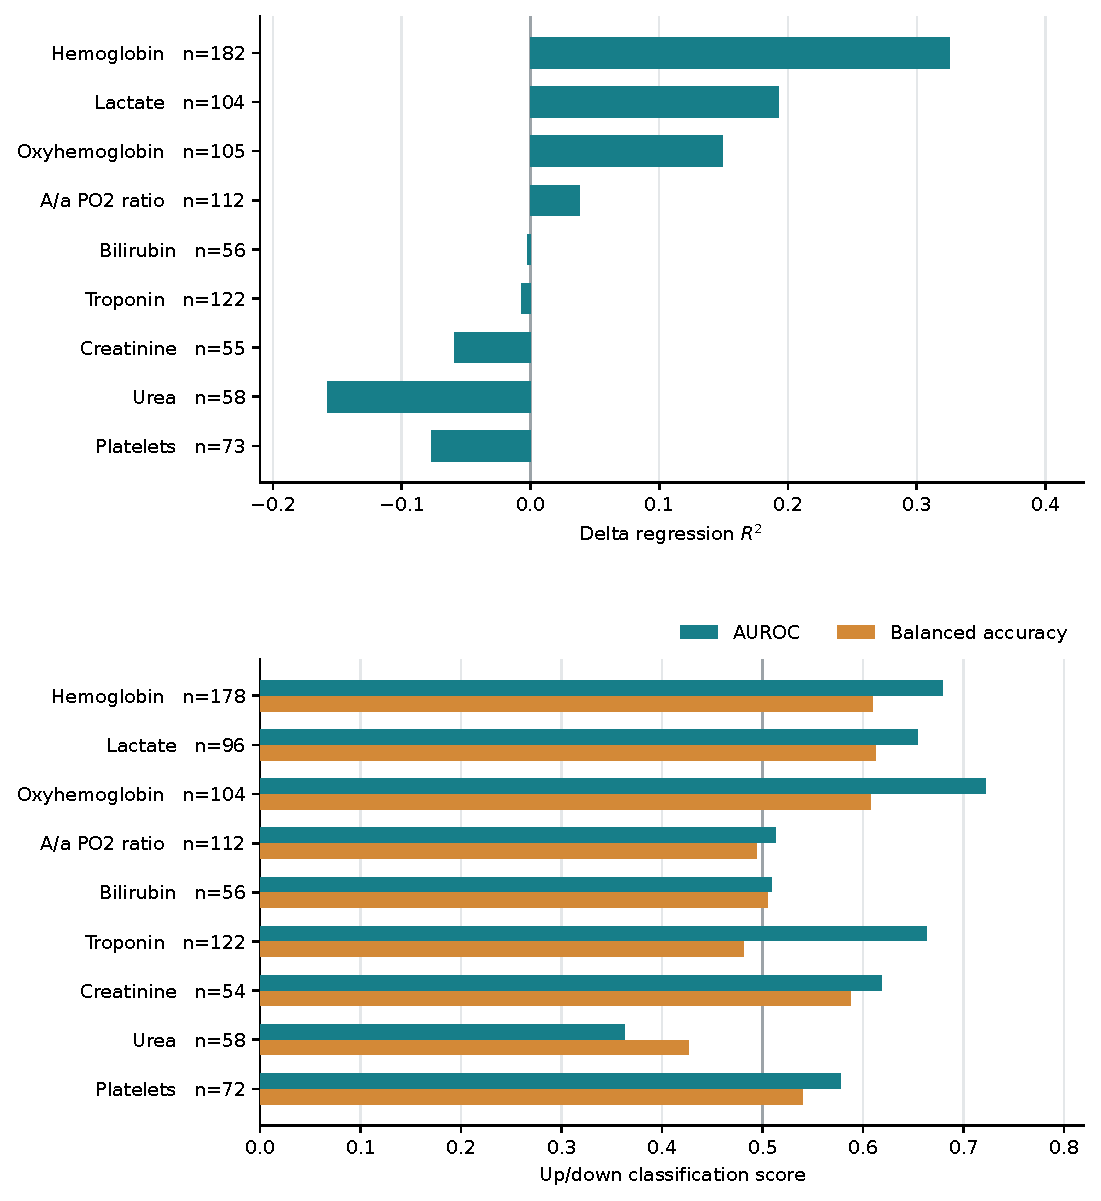
\includegraphics[width=0.90\linewidth]{figures/exp6_delta_tasks.pdf}
\caption{Original held-out pair-level regression and separately trained direction-classification results. The panels display their own sample counts.}
\label{fig:change}
\end{figure}

Figure~\ref{fig:predtrue} compares observed and predicted hemoglobin for original held-out single-video and paired-change cohorts. Fits cover only observed test-value ranges. The frozen-feature analysis yielded median target-wise Spearman $\rho$ of $0.073$ for face-only features, $0.048$ for face features from the fusion model, and $0.033$ for paired feature differences. Four source--target tests had within-family adjusted $q<0.05$; the largest reported $\rho$ among them was $0.278$ for face-only bilirubin.

\noindent\begin{minipage}{\linewidth}
\centering
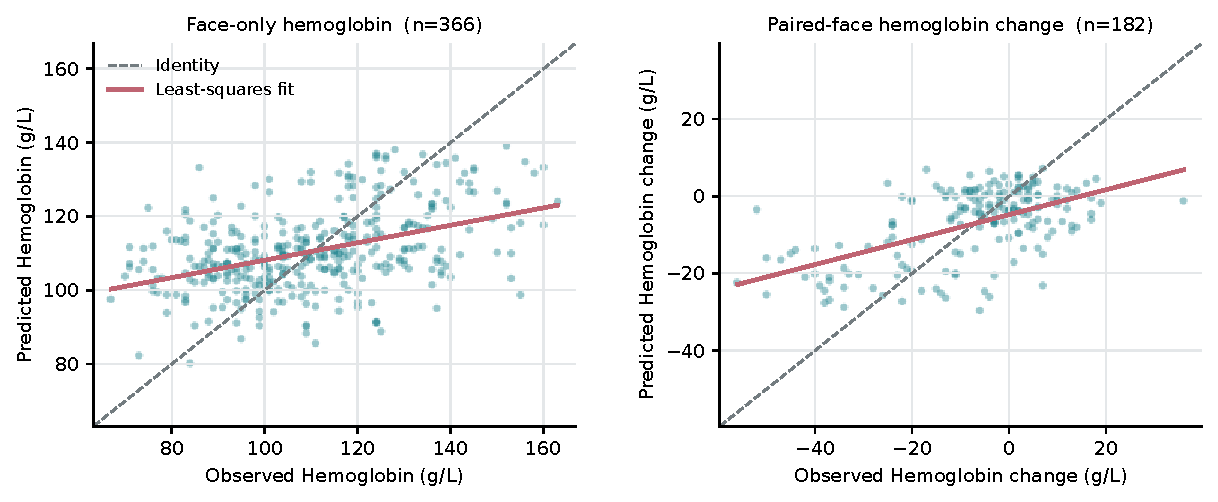
\includegraphics[width=0.85\linewidth]{figures/hemoglobin_predicted_vs_true.pdf}
\captionof{figure}{Observed versus predicted hemoglobin for absolute-value regression (left) and ordered-pair change regression (right), each on its original held-out test set. Dashed gray lines indicate identity; solid rose lines are least-squares fits.}
\label{fig:predtrue}
\end{minipage}

\section{Study 4: Postoperative status from facial recordings}

\subsection{Target definitions and protocols}

Valid CABG hospitalizations supplied surgery and discharge times. The first target was a constructed recovery-time fraction: zero at CABG completion and one at discharge, linearly interpolated at postoperative video time. Laboratory values were not part of this target. The other two targets used postoperative laboratory reports: a nine-analyte trajectory-deviation score and a four-item partial-CASUS subtotal. Their configurations were:
\begin{itemize}
\setlength{\itemsep}{1pt}
\item \textbf{Time-defined recovery:} complete videos between CABG end and discharge, with a distribution-selected, patient-disjoint 60/20/20 split. Input comprised 20 nonadjacent face frames and five training views. ImageNet-pretrained EfficientNet-B0 had a 32-unit sigmoid head. The frozen-encoder head stage used learning rate $10^{-3}$; later only the final encoder stage was unfrozen, with backbone/head rates $10^{-5}/10^{-4}$. Patient-balanced Smooth L1 training was evaluated by averaging 20 original-frame predictions per video.
\item \textbf{Postoperative trajectory deviation:} the equal-weight mean of nine absolute residuals from training-patient median postoperative trajectories, each divided by the local IQR. The analytes were lactate, troponin I, creatinine, total bilirubin, platelets, hemoglobin, C-reactive protein, albumin, and PaO$_2$. Only strictly postoperative reports entered trajectory fitting and label matching; all nine results had to be available within 24 hours. Pre/postoperative models used separate ImageNet-pretrained EfficientNet-B0 encoders, 64-unit projectors, and a 32-unit fusion head. The frozen-encoder head stage used $2\times10^{-4}$ for up to 30 epochs; last-stage fine-tuning used backbone/head rates $10^{-5}/10^{-4}$ for up to 50, with patience 8/10. Pre-only and post-only protocols used their own maximum eligible cohorts.
\item \textbf{Partial CASUS:} a 0--16-point subtotal from creatinine, bilirubin, lactate, and platelets, requiring all four 24-hour matches. The paired-face model used the independent-encoder architecture above, 20 nonadjacent frames and three training views; a post-face-only variant retained the same outcome and used all eligible postoperative videos. Training divided the target by 16 for its sigmoid output; reported errors were returned to score points. This four-item subtotal is not the full CASUS score.
\end{itemize}

\begin{center}
\begin{minipage}{\linewidth}
\centering
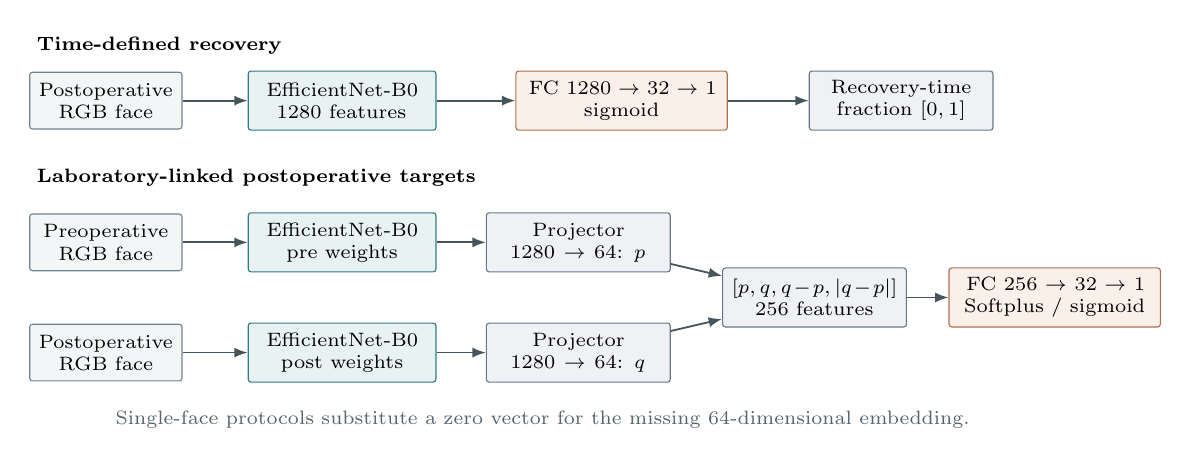
\begin{tikzpicture}[
    x=1cm,y=1cm,>=Latex,
    every node/.style={font=\scriptsize,align=center},
    source/.style={draw=diagramSource,fill=diagramSourceBg,rounded corners=1pt,minimum height=0.72cm,text width=1.7cm},
    encoder/.style={draw=diagramEncoder,fill=diagramEncoderBg,rounded corners=1pt,minimum height=0.75cm,text width=2.15cm},
    op/.style={draw=diagramOp,fill=diagramOpBg,rounded corners=1pt,minimum height=0.75cm,text width=2.1cm},
    head/.style={draw=diagramHead,fill=diagramHeadBg,rounded corners=1pt,minimum height=0.75cm,text width=2.45cm},
    flow/.style={-{Latex[length=1.7mm]},draw=diagramFlow,line width=0.65pt}
]
\node[anchor=west,font=\bfseries\scriptsize] at (0,3.4) {Time-defined recovery};
\node[source] (single) at (1.0,2.7) {Postoperative\\RGB face};
\node[encoder] (singleenc) at (4.0,2.7) {EfficientNet-B0\\1280 features};
\node[head] (singlehead) at (7.55,2.7) {FC $1280\to32\to1$\\sigmoid};
\node[op] (time) at (11.1,2.7) {Recovery-time\\fraction $[0,1]$};
\draw[flow] (single) -- (singleenc);
\draw[flow] (singleenc) -- (singlehead);
\draw[flow] (singlehead) -- (time);

\node[anchor=west,font=\bfseries\scriptsize] at (0,1.72) {Laboratory-linked postoperative targets};
\node[source] (pre) at (1.0,0.90) {Preoperative\\RGB face};
\node[source] (post) at (1.0,-0.50) {Postoperative\\RGB face};
\node[encoder] (preenc) at (4.0,0.90) {EfficientNet-B0\\pre weights};
\node[encoder] (postenc) at (4.0,-0.50) {EfficientNet-B0\\post weights};
\node[op] (preproj) at (7.0,0.90) {Projector\\$1280\to64$: $p$};
\node[op] (postproj) at (7.0,-0.50) {Projector\\$1280\to64$: $q$};
\node[op] (fuse) at (10.0,0.20) {$[p,q,q-p,|q-p|]$\\256 features};
\node[head] (pairhead) at (13.05,0.20) {FC $256\to32\to1$\\Softplus / sigmoid};
\draw[flow] (pre) -- (preenc);
\draw[flow] (post) -- (postenc);
\draw[flow] (preenc) -- (preproj);
\draw[flow] (postenc) -- (postproj);
\draw[flow] (preproj) -- (fuse);
\draw[flow] (postproj) -- (fuse);
\draw[flow] (fuse) -- (pairhead);
\node[anchor=west,font=\scriptsize,text=diagramNote] at (1.0,-1.35)
    {Single-face protocols substitute a zero vector for the missing 64-dimensional embedding.};
\end{tikzpicture}

\captionof{figure}{Study 4 architectures. The constructed recovery-time target uses one face encoder. Laboratory-linked paired models have independently trainable pre/postoperative encoders and concatenate their projected features and differences. The trajectory-deviation head uses Softplus; the partial-CASUS head uses sigmoid after scaling the score to $[0,1]$. Single-face protocols set the absent projected feature to zero.}
\label{fig:postoparch}
\end{minipage}
\end{center}

All postoperative metrics used patient-disjoint held-out sets. The paired partial-CASUS result used an earlier laboratory-table snapshot than the post-face-only partial-CASUS result. Moreover, the pre-only, post-only, and pair trajectory-deviation protocols had different eligible cohorts; neither comparison is a matched ablation.

\subsection{Held-out performance}

The time-defined recovery target was evaluated on 274 videos, with MAE $0.177$ on its 0--1 scale, $R^2=0.135$, and Pearson $r=0.416$. The nine-analyte trajectory-deviation target yielded test $R^2=0.139$ and $r=0.398$ on 73 paired-face videos. Pre-only and post-only protocols evaluated 67 and 78 videos, with $R^2=-0.098$ and $-0.122$. The earlier-snapshot paired partial-CASUS model had $R^2=-0.002$ on 58 videos. The current-snapshot post-face-only partial-CASUS model had $R^2=-0.110$ on 85 videos. These postoperative endpoints and source snapshots should be interpreted separately.

\section{Study 5: ECG signal-quality control}

An independent ECG branch used raw signal windows and generated targets for QRS reliability and waveform morphology. ResNet and temporal-convolutional-network encoders were compared with window-derived and reference-beat templates. The weak-label training configuration used 10-second windows, a one-second step, 1,024-point inputs, a 20\% validation fraction, batch size 32, and a frozen pretrained encoder. The head used a learning rate of $5\times10^{-4}$, weight decay $10^{-4}$, and at most 50 epochs. Natural ECG files lacked human signal-quality annotations, so validation against generated targets and sensitivity to controlled corruptions cannot establish clinical classification accuracy.

\begin{center}
\begin{minipage}{\linewidth}
\centering
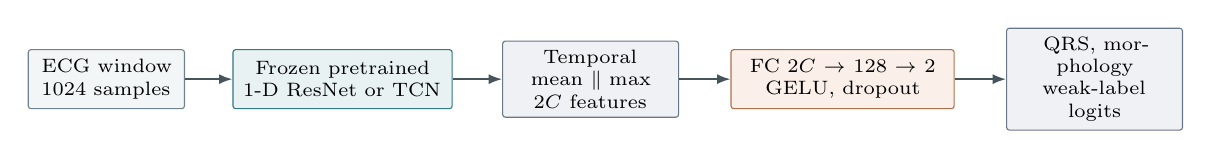
\begin{tikzpicture}[
    x=1cm,y=1cm,>=Latex,
    every node/.style={font=\scriptsize,align=center},
    source/.style={draw=diagramSource,fill=diagramSourceBg,rounded corners=1pt,minimum height=0.75cm,text width=1.75cm},
    encoder/.style={draw=diagramEncoder,fill=diagramEncoderBg,rounded corners=1pt,minimum height=0.75cm,text width=2.55cm},
    op/.style={draw=diagramOp,fill=diagramOpBg,rounded corners=1pt,minimum height=0.75cm,text width=2.0cm},
    head/.style={draw=diagramHead,fill=diagramHeadBg,rounded corners=1pt,minimum height=0.75cm,text width=2.6cm},
    flow/.style={-{Latex[length=1.7mm]},draw=diagramFlow,line width=0.65pt}
]
\node[source] (signal) at (1.0,0) {ECG window\\1024 samples};
\node[encoder] (enc) at (4.0,0) {Frozen pretrained\\1-D ResNet or TCN};
\node[op] (pool) at (7.15,0) {Temporal mean $\Vert$ max\\$2C$ features};
\node[head] (head) at (10.35,0) {FC $2C\to128\to2$\\GELU, dropout};
\node[op] (target) at (13.55,0) {QRS, morphology\\weak-label logits};
\draw[flow] (signal) -- (enc);
\draw[flow] (enc) -- (pool);
\draw[flow] (pool) -- (head);
\draw[flow] (head) -- (target);
\end{tikzpicture}

\captionof{figure}{Study 5 weak-label ECG model. A pretrained one-dimensional encoder is frozen; temporal mean and maximum features are concatenated before a two-logit quality head. ResNet and TCN are alternative encoders, not simultaneous branches.}
\label{fig:ecgarch}
\end{minipage}
\end{center}

The raw-data evaluation covered 7,587 windows from 2,592 patient files. On weak-label validation, the temporal-convolutional window-template variant achieved AUROC $0.998$ for QRS reliability and $0.997$ for morphology; the ResNet window-template variant achieved $0.887$ and $0.884$. Response to severe corruption depended on its type and on the model. These figures are agreement with generated targets, not accuracy against expert annotations, and neither the source nor the statistical unit was comparable to the face-video studies.

\end{document}
